% Upcrossings of [a,b] by a random walk path, with the holding periods of the buy-low-sell-high strategy shaded. Generated by a short script.
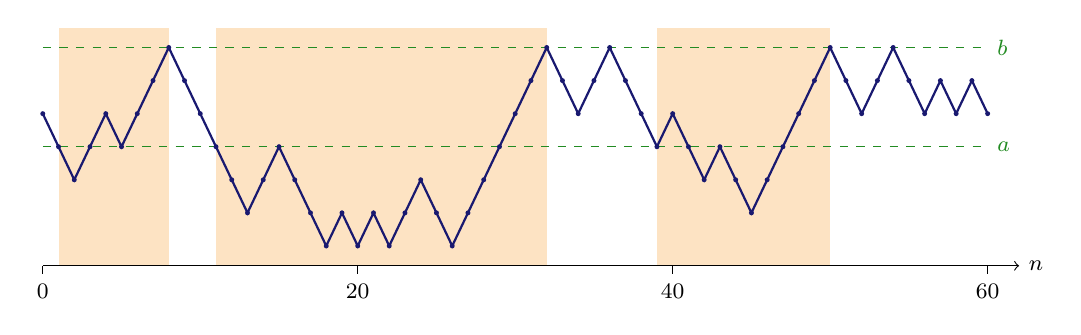
\begin{tikzpicture}[x=0.2cm,y=0.42cm,every node/.style={font=\footnotesize}]
\fill[BurntOrange!20] (1,-4.6) rectangle (8,2.6);
\fill[BurntOrange!20] (11,-4.6) rectangle (32,2.6);
\fill[BurntOrange!20] (39,-4.6) rectangle (50,2.6);
\draw[->] (0,-4.6)--(62,-4.6) node[right] {$n$};
\draw (0,-4.6)--(0,-4.85) node[below] {$0$};
\draw (20,-4.6)--(20,-4.85) node[below] {$20$};
\draw (40,-4.6)--(40,-4.85) node[below] {$40$};
\draw (60,-4.6)--(60,-4.85) node[below] {$60$};
\draw[ForestGreen,dashed] (0,-1)--(60,-1) node[right] {$a$};
\draw[ForestGreen,dashed] (0,2)--(60,2) node[right] {$b$};
\draw[MidnightBlue,thick] (0,0)--(1,-1)--(2,-2)--(3,-1)--(4,0)--(5,-1)--(6,0)--(7,1)--(8,2)--(9,1)--(10,0)--(11,-1)--(12,-2)--(13,-3)--(14,-2)--(15,-1)--(16,-2)--(17,-3)--(18,-4)--(19,-3)--(20,-4)--(21,-3)--(22,-4)--(23,-3)--(24,-2)--(25,-3)--(26,-4)--(27,-3)--(28,-2)--(29,-1)--(30,0)--(31,1)--(32,2)--(33,1)--(34,0)--(35,1)--(36,2)--(37,1)--(38,0)--(39,-1)--(40,0)--(41,-1)--(42,-2)--(43,-1)--(44,-2)--(45,-3)--(46,-2)--(47,-1)--(48,0)--(49,1)--(50,2)--(51,1)--(52,0)--(53,1)--(54,2)--(55,1)--(56,0)--(57,1)--(58,0)--(59,1)--(60,0);
\fill[MidnightBlue] (0,0) circle (0.9pt);
\fill[MidnightBlue] (1,-1) circle (0.9pt);
\fill[MidnightBlue] (2,-2) circle (0.9pt);
\fill[MidnightBlue] (3,-1) circle (0.9pt);
\fill[MidnightBlue] (4,0) circle (0.9pt);
\fill[MidnightBlue] (5,-1) circle (0.9pt);
\fill[MidnightBlue] (6,0) circle (0.9pt);
\fill[MidnightBlue] (7,1) circle (0.9pt);
\fill[MidnightBlue] (8,2) circle (0.9pt);
\fill[MidnightBlue] (9,1) circle (0.9pt);
\fill[MidnightBlue] (10,0) circle (0.9pt);
\fill[MidnightBlue] (11,-1) circle (0.9pt);
\fill[MidnightBlue] (12,-2) circle (0.9pt);
\fill[MidnightBlue] (13,-3) circle (0.9pt);
\fill[MidnightBlue] (14,-2) circle (0.9pt);
\fill[MidnightBlue] (15,-1) circle (0.9pt);
\fill[MidnightBlue] (16,-2) circle (0.9pt);
\fill[MidnightBlue] (17,-3) circle (0.9pt);
\fill[MidnightBlue] (18,-4) circle (0.9pt);
\fill[MidnightBlue] (19,-3) circle (0.9pt);
\fill[MidnightBlue] (20,-4) circle (0.9pt);
\fill[MidnightBlue] (21,-3) circle (0.9pt);
\fill[MidnightBlue] (22,-4) circle (0.9pt);
\fill[MidnightBlue] (23,-3) circle (0.9pt);
\fill[MidnightBlue] (24,-2) circle (0.9pt);
\fill[MidnightBlue] (25,-3) circle (0.9pt);
\fill[MidnightBlue] (26,-4) circle (0.9pt);
\fill[MidnightBlue] (27,-3) circle (0.9pt);
\fill[MidnightBlue] (28,-2) circle (0.9pt);
\fill[MidnightBlue] (29,-1) circle (0.9pt);
\fill[MidnightBlue] (30,0) circle (0.9pt);
\fill[MidnightBlue] (31,1) circle (0.9pt);
\fill[MidnightBlue] (32,2) circle (0.9pt);
\fill[MidnightBlue] (33,1) circle (0.9pt);
\fill[MidnightBlue] (34,0) circle (0.9pt);
\fill[MidnightBlue] (35,1) circle (0.9pt);
\fill[MidnightBlue] (36,2) circle (0.9pt);
\fill[MidnightBlue] (37,1) circle (0.9pt);
\fill[MidnightBlue] (38,0) circle (0.9pt);
\fill[MidnightBlue] (39,-1) circle (0.9pt);
\fill[MidnightBlue] (40,0) circle (0.9pt);
\fill[MidnightBlue] (41,-1) circle (0.9pt);
\fill[MidnightBlue] (42,-2) circle (0.9pt);
\fill[MidnightBlue] (43,-1) circle (0.9pt);
\fill[MidnightBlue] (44,-2) circle (0.9pt);
\fill[MidnightBlue] (45,-3) circle (0.9pt);
\fill[MidnightBlue] (46,-2) circle (0.9pt);
\fill[MidnightBlue] (47,-1) circle (0.9pt);
\fill[MidnightBlue] (48,0) circle (0.9pt);
\fill[MidnightBlue] (49,1) circle (0.9pt);
\fill[MidnightBlue] (50,2) circle (0.9pt);
\fill[MidnightBlue] (51,1) circle (0.9pt);
\fill[MidnightBlue] (52,0) circle (0.9pt);
\fill[MidnightBlue] (53,1) circle (0.9pt);
\fill[MidnightBlue] (54,2) circle (0.9pt);
\fill[MidnightBlue] (55,1) circle (0.9pt);
\fill[MidnightBlue] (56,0) circle (0.9pt);
\fill[MidnightBlue] (57,1) circle (0.9pt);
\fill[MidnightBlue] (58,0) circle (0.9pt);
\fill[MidnightBlue] (59,1) circle (0.9pt);
\fill[MidnightBlue] (60,0) circle (0.9pt);
\end{tikzpicture}
